\section{Transformation of an SDN network to an OpenFlow switch}
\label{Sec:Design}

\begin{comment}
The overview of our model abstraction approach for SDN networks is shown in Figure~\ref{Fig:BigSimOverview}. Through a three-step systematic process, we are able to take 
a snapshot of an SDN network $SN$ as the input, transform the network devices in an SDN network to a single OpenFlow switch, $BS$ that preserves the forwarding logic of the original network. In this section, we elaborate the algorithmic design in each step of the model abstraction.
%We have sketched the process of how to replace a OpenFlow-switch-connected network with a single OpenFlow switch in section~\ref{Sec:MotivationalExample}.
\end{comment}

Our objective is to take a static SDN dataplane configuration (i.e., a snapshot) and transform it to a single ``big switch", which preserves the same end-to-end forwarding behavior. In other words, if a packet originated from a host is forwarded to host in the snapshot, then the packet will be sent to the same destination by the ``big switch". So, the essential task is to (1) identify how every possible packet is processed by the snapshot and (2) correctly configure the ``big switch" so that every packet is processed the same way. We developed a three-step approach to accomplish this task, as shown in Figure \ref{Fig:BigSimOverview}:

\begin{itemize}
\item Find Equivalence Classes: We borrow the concept of Equivalence Class (EC) from VeriFlow\cite{Veriflow}, which enables us to partition all possible packets in the network into mutually exclusive sets, such that packets belongs to the same set are processed in the same way. ECs are identified according to the match field of \textbf{all} the OpenFlow rules on \textbf{all} the switches in the network.
\item Traverse Forwarding Graphs: After partitioning the packets into ECs, we study the behavior of each individual EC using the topology information and the switch local information (port mapping, rule priorities, etc), and generate forwarding graphs to represent the behavior.  
\item Generate OpenFlow Rules: Finally, we generate the OpenFlow rules on the ``big switch" to preserve the same end-to-end behavior. This step includes (1) construct the port-to-host mapping and (2) generate the rules by matching the header of each EC and forward to the correct output port, which is decided by traversing the forwarding graph acquired by the last step.
\end{itemize}

Our three-step approach is able to correctly transform based on two assumptions. First, although the SDN network contains the control plane and the dateplane, and the configuration of each network devices can be dynamically changed by the controller, we assume the frequency of control messages are far less than the rate of the incoming packets. So between two configuration updates, the dataplane is fixed. Thus we don't need to include the controller into our model abstraction to preserve the forwarding behavior. Second, the packet processing of the SDN devices is assumed to be simple. For example, in this work we assume both the original network and ``big switch" use OpenFlow switches, which apply a simple scheme that is to match the incoming packet to the rule with highest priority and then apply the action of that rule. The simplicity of OpenFlow switches enables us to analyze the behavior of the original network and synthesis the configuration of the ``big switch". We describe each step in detail in the following subsections.
   
\subsection{Identifying Equivalent Classes}
\begin{comment}
By aggregating and slicing forwarding rules in an SDN network according to ECs, one can obtain a compact representation of the network state in terms of forwarding behavior. 
\end{comment}

We first give the definition of equivalence class (EC), and then present the data structure and algorithms to partition the packets into ECs in the network.

\begin{definition}
An equivalence class (EC) is a set of packets that experience the identical forwarding action at \textbf{any} network device in the network. 
\label{Def:EC}
\end{definition}

\begin{comment}
%\kevin{add to one or two sentences about how to find ECs and how to aggregate ECs before the structure}
By its definition, ECs can be found by aggregate forwarding rules on different switches
and group them by the match field.
We aggregate forwarding rules using a trie structure as inspired by VeriFlow\cite{Veriflow}. 
A trie node has three child nodes, i.e., zero, one or wildcard, that represent three possible values for performing a bit-to-bit rule matching.
The entire tree is composited by several sub-tries, each representing one packet header field. For example, consider the tree-topology network in Section \ref{Sec:MotivatingExample}, the trie only contains one sub-trie representing the $NW\_DST$ header field (i.e., the network destination address). Note that an EC can be defined by multiple fields. For example, we can also match the source address of the packet (e.g., $NW\_SRC$) as well as the service type of the traffic ($TCP\_SRC$). The resulting trie now has three sub-tries.
%Here we give solutions to two problems that VeriFlow neglected.
\end{comment}

Each packet is uniquely identified by its header values, According to OpenFlow specification, 


\subsubsection{Disjoint Equivalent Classes}
By traversing from the root node to a leaf node, we can obtain a set of packets that a rule matches.
Therefore, the leaves contain all the packet header values in the network,
paired as a series of ranges\footnote{In this text, the word ``interval" is used interchangeably with ``range"},
as $A, B$ and $C$ in Figure~\ref{Fig:DisjointECsAsInterval}.
These header value ranges are not independent and may overlap with each other.
Finding the set of disjoint ECs requires us to split this list of ranges $R$ to a list of non-overlapping intervals. The result is a set of disjoint ECs as shown in the upper part of Figure~\ref{Fig:DisjointECsAsInterval}. 
We develop Algorithm~\ref{Alg:GenDisjointECs} to generate a set of disjoint ECs and show that the generation can be accomplished in $O(N \times M\log M)$ time,
where $M=|R|$ is the number of intervals and $N$ is the number of header bits.
% as follows\cite{SplitDisjointInterval}.
%Not algorithmic described in\cite{Veriflow},

First, we place $R$ into an array $A$ of $2M$ values,
each flagged as either a start point, or an end point, of a range
\footnote{Equal values with same flag are reduced to an single element.}.
Before iterating $A$, we sort it, breaking the tie by putting start point before end point.
Then we maintain the difference $d$ between the number of seen start points and
the number of seen end points. While visit each point in sorted order:
\begin{itemize}
\item If the current element $x \in S$ and $d > 0$,
        we end the previous interval with the ending value $x - 1$;
        Start a new interval with a starting value $x$
        (line~\ref{Alg:LineEndStart1}-\ref{Alg:LineEndStart2}).
\item If the current element $x \in E$, we end the previous interval with the ending value $x$.
        (line~\ref{Alg:LineEndEnd}).
\item In either case, we update the potential new interval's start value \textit{prev}
        (line~\ref{Alg:LineNewPrev1} and \ref{Alg:LineNewPrev2}).
\end{itemize}

Updating forwarding rules in the network will change the EC set.
By maintaining the rules in a trie, we can efficiently update ECs in an incremental way. An insertion of a new rule requires us to do a depth-first-style trie traverse. This process automatically narrows down the set of affected rules by ignoring those non-overlapping branches with the new rule.
The output is the set of the affected ranges, and we need to run Algorithm~\ref{Alg:GenDisjointECs} to update ECs only in the affected ranges.


\begin{figure}[t]
\centering
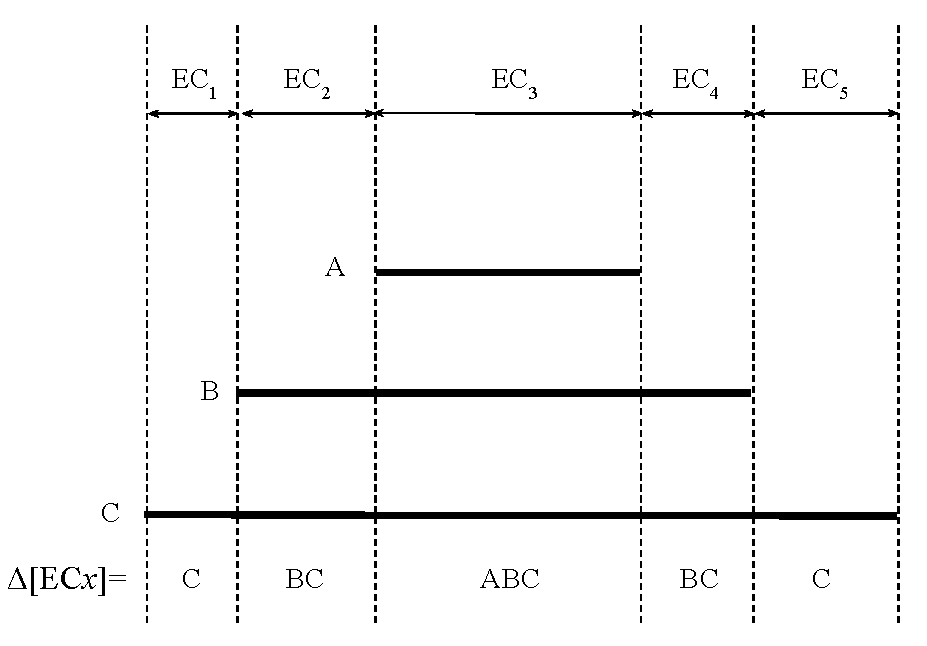
\includegraphics[scale=.52]{figures/DisjointECs.pdf}
\caption{A class of packets are abstracted as a range of packet header values.
        Five equivalence classes, shown at the top, can be obtained via splitting three ranges A, B and C.
        Finding $\Delta[EC_x]$, the rules that intersect with EC $x$, is instrumental for
        merge equivalent ECs, which are shown at the bottom.}
\label{Fig:DisjointECsAsInterval}
\end{figure}

\begin{algorithm}[t]
\DontPrintSemicolon
\KwData{$R = $ a set of rules from the leaf-node of the trie}
\KwResult{$EC = $ a set of equivalence classes as disjoint intervals}
$cnt \gets 0$\;
$S = $ \{starting points of $\forall r \in R\}$, $E = $ \{end points of $\forall r \in R\}$\;
$A \gets Sort(S \bigcup E)$ in non-decreasing order\;
$EC \gets \emptyset$\;
\ForEach {$x \in A$} {
        \uIf {$x \in S$} {
                \If {$cnt \neq 0$} {\label{Alg:LineEndStart1} 
                        $EC \gets EC \text{ }\bigcup \text{} [prev, x-1]$\;
                }\label{Alg:LineEndStart2} 
                $prev \gets x$\;\label{Alg:LineNewPrev1}
                $cnt \gets cnt + 1$\;
        }
        \Else ($x \in E$) {
                $EC \gets EC \text{ } \bigcup \text{ } [prev, x]$\;\label{Alg:LineEndEnd}
                $prev \gets x + 1$\;\label{Alg:LineNewPrev2}
                $cnt \gets cnt - 1$\;
        }
}
\caption{Generate Disjoint ECs}
\label{Alg:GenDisjointECs}
\end{algorithm}

\subsubsection{Union Equivalent Classes}
The disjoint EC set $ECS$ obtained from Algorithm~\ref{Alg:GenDisjointECs} are not the optimal one. 
We can merge some ECs if they represent the identical packet forwarding behavior (see the definition of ECs). 
For example, $EC_2$ and $EC_4$ in Figure~\ref{Fig:DisjointECsAsInterval} can be merged as one EC, since the packets in both ECs experience the same set of forwarding rules throughout the network. %To generate the correct set of rules on the new ``big switch", we only need to model the forwarding behavior of either one of the ECs. In other words, for any two ECs $\alpha$ and $\beta$, we have:

\begin{lemma}
$\forall \alpha, \beta $ if $\alpha$ and $\beta$ are mergeable, then $FG(\alpha) \equiv FG(\beta)$.
\label{Lemma:MergeFG}
\end{lemma}
$FG()$ in Lemma~\ref{Lemma:MergeFG} is a function that maps an EC into a forwarding graph, which will be defined and illustrated in Section \ref{Sec:Generating Forwarding Graphs}. In fact, using the minimal EC set can significantly reduce the running time in the next two phases: generating forwarding graph and populating final OpenFlow rules. Here we provide a solution, which builds on the following lemma.

\begin{lemma}
For any two disjoint ECs $\alpha$ and $\beta$, they are mergeable
if they intersect with the same set of rules $\Delta$ in the network.
\label{Lemma:MergeEC}
\end{lemma}
%According to Lemma~\ref{Lemma:MergeEC}, 
For example, both $EC_2$ and $EC_4$ intersect with range $B$ and $C$ in Figure~\ref{Fig:DisjointECsAsInterval}, and therefore, we can treat them as one EC.

If EC $\alpha$ and EC $\beta$ satisfy the condition in Lemma~\ref{Lemma:MergeEC},
$\alpha$ and $\beta$ are derived from the same set of rules according to Algorithm~\ref{Alg:GenDisjointECs}.
For any network device $d$, let $\delta \in \Delta$ be the rule on $d$ with the highest priority.
If no such $\delta$ exists, packets from both $\alpha$ and $\beta$ are dropped on $d$.
Otherwise, packets in both $\alpha$ and $\beta$ match rule $\delta$, and
device $d$ will forward both of them according to the action specified in $\delta$.
Note that in another device $d'$, the highest priority rule that covers both $\alpha$
and $\beta$ may be different, i.e., $\delta' \neq \delta$.
However, as long as $\delta$ is unique at given $d$, the forwarding behavior at $d$ for both $\alpha$ and $\beta$ are always identical.
By Definition~\ref{Def:EC}, packets in $\alpha$ and $\beta$ can be merged as one single EC.

We can efficiently find the list of rules $\Delta[\alpha]$ that intersect with EC $\alpha$ using two data structures: an array of pointers and a central interval tree.
Each of them is responsible for one of the two cases \cite{FindIntersectionWiki}.
\begin{itemize}
\item Case 1: Rule $\delta$ intersects $\alpha$ with its starting and/or end point in $\alpha$.
        We can reuse the sorted array $A$ in Algorithm~\ref{Alg:GenDisjointECs}.
        We augment each value, either a start point or a end point of an range, in $A$
        with a pointer to the rule that the value belongs to.
        By doing a binary search, we can find the minimum and maximum values in $A$,
        which bound the range of $\alpha$.
        All intervals that intersect with $\alpha$ must be between the minima and maxima,
        meaning we can ignore two kinds of rules: these whose end point is
        smaller than minima and these whose start point is larger than maxima.
        We then perform a linear search in the size-reduced set of rules,
        check one by one if the range intersects with $\alpha$.
        The total time complexity for both linear search and binary search are $O(\log M + K)$,
        where $K=|\Delta|$ is the number of reported intervals.
\item Case 2: Rule $\delta$ covers $\alpha$ entirely. We can build
        a central interval tree\cite{ComputationalGeometryBook} using all the available ranges.
        We pick a random value $x \in \alpha$ and query the central interval tree for
        all the ranges that intersect with $x$, which can be done in $O(\log M + K)$ time,
        at the cost of $O(M log M)$ time for building the central interval tree.
        Since central interval tree support efficient incremental operations (insertion and deletion),
        dynamic changes of rule set are also supported.
\end{itemize}

Using both the interval tree and ordered list, for each EC $\alpha$,
we find the list of intervals $\Delta[\alpha]$ that intersect with $\alpha$.
By mapping each rule $\delta \in \Delta$ to a unique binary ID $c_\delta$ of length $\log_2 M$,
we can encode $\Delta[\alpha]$ to a string of $c_\delta$s, putting small ID at front.
This string of unique IDs, named $C_\alpha$, is of at most length $M\log_2 M$.
We then use a hash table $H$ to group the mergeable ECs by hashing each EC $x$ to $C_x$.
The minimal size of ECs is the number of unique keys in $H$.
Note that in the subsequent algorithmic designs, iterating through all (disjoint) ECs refers to iterating through the first ECs in each set $H[key]$.%, $\forall key \in H$.

\subsection{Generating Forwarding Graphs}
\label{Sec:Generating Forwarding Graphs}

In the second step, we compute a forwarding graph for each EC, and then effectively reduce the size of the forwarding graph to improve efficiency for the third step. 

A forwarding graph is a directed graph that represents how packets belonging to the same EC are processed by the network. A node $u$ in the forwarding graph is a networking device, and an edge $(u, v)$ in the graph means that device $u$ forwards the packets to device $v$ in the network. 
A forwarding graph not only concatenates the forwarding behavior for each EC, but also visualizes the data flow of the EC in the network. 
%For a fixed EC $x$, we connect the network devices that have rules for $x$ with directed edges that point to the next hop, which is determined by the action field of the rule.
Since our objective is to abstract the network forwarding logic into a big switch, our end-to-end modeling focuses on the sources and sinks of the graph. 
Figure~\ref{Fig:ForwardingGraphECX} depicts the generalized forwarding graph $FG(x)$ for EC $x$. 
 
%Here we discuss two specific issues in the forwarding graph generation: where to start the traversal according to our needs and what we can achieve at the end of the traversal.

\begin{figure*}[t]
\centering
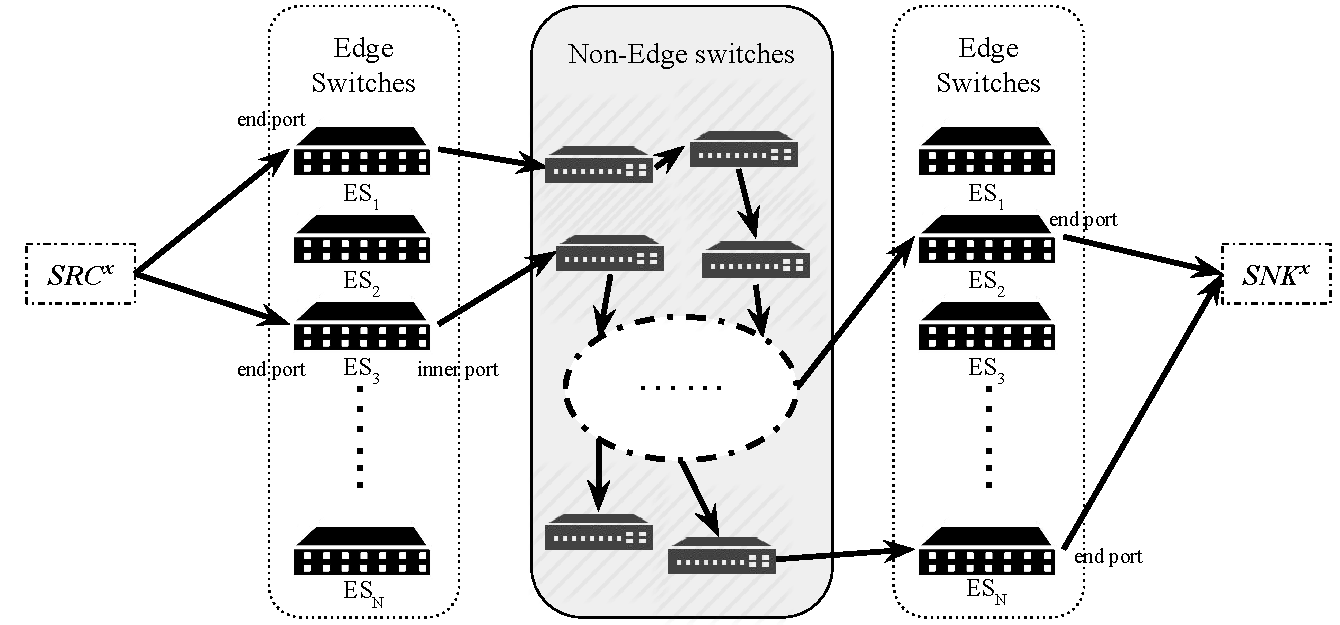
\includegraphics[scale=.75]{figures/ForwardingGraph.pdf}
\caption{Modeling a Forwarding Graph of an Equivalent Class}
\label{Fig:ForwardingGraphECX}
\end{figure*}

\subsubsection{Network Traversal for Forwarding Graph Generation}

We develop a forwarding graph generation algorithm as shown in Algorithm~\ref{Alg:GenForwardingGraph}.
The notations are defined as follows.
$FG(x)$ denotes the forwarding graph for a particular equivalent class x.
A \textit{edge switch} is defined as a switch that has at least one link to a node outside $SN$.
A \textit{non-edge switch} is defined as a switch whose connected nodes are all inside $SN$.
The forwarding behavior of the non-edge switches are remove in the big switch abstraction.
$src$ denotes the source node of the forwarding path for an EC,
and $snk$ denotes the sink node of the forwarding path for an EC.
Note that all $src$ in $FG(x)$ are edge switches,
and $snk$ in $FG(x)$ can be either edge switches or non-edge switches.
$curr$ denotes the current node in the network that we are traversing to generate the forwarding graph.
We add a super-source node, $SRC^x$, and a super-sink node, $SNK^x$, as the boundaries of $FG(x)$.

Algorithm~\ref{Alg:GenForwardingGraph} is designed to generate $FG(x)$.
We start the process from each $src$ that connects to $SRC^x$,
and then traverse EC $x$'s forwarding graph using depth-first-based-search and
follow the action specified in the highest-priority forwarding rule for EC $x$ at each node along the way. 

%(2) the inner graph may contain both edge and internal switches.
%Source node $src$ and its out-going edge represent an edge switch $sw$ that forwards EC $x$ \textbf{coming from} port $p$; it can be described by $(sw, p)$ pair. Sink node $snk$ represent the end of the forwarding $sw$, which is also denoted by $(sw, p)$, where $p$ is either the port number specified by the action field or \texttt{NULL} if there is no rule for $x$ on $sw$.
%We denote the set of source nodes as $SRC(x)$, the set of sink nodes as $SNK(x)$.

We distinguish two kinds of port on an edge switch:
\begin{itemize}
\item \textit{end port} that connects to a node that is either the forwarding end point or outside the network one wants to abstract
\item \textit{inner port} that connects to a node inside the network that one wants to abstract.
\end{itemize}

We add an edge from $SRC^x$ to a $src$, if the source node has a forwarding rule $r$ that matches EC $x$, or the $IN\_PORT$ field of rule $r$ on the source node is an end port. 
Otherwise, we do not need to initiate a traverse (see line~\ref{Alg:LineStartDFS1} to~\ref{Alg:LineStartDFS2} in Algorithm~\ref{Alg:GenForwardingGraph}).
Correspondingly, we add an edge from a $snk$ to the super sink $SNK^x$ if both conditions are satisfied:
\begin{enumerate}
\item the sink node is an edge switch in the network;
\item the $OUT\_PORT$ field determined by the rule's action on the sink node is an end port.
\end{enumerate}

\begin{algorithm}[h]
\DontPrintSemicolon
\KwIn{$nodes = $ Switches containing rules for EC $x$ \newline
        $topo = $ Network topology}
\KwResult{Forwarding graph $FG(x)$ for EC $x$}
\SetKwProg{Fn}{Function}{}{\KwRet}
\SetKwFunction{Traverse}{traverse}
\SetKwFunction{GenRule}{generate\_rules}
\Fn{\Traverse{$curr$, $src$, $snk$}} {
        \uIf {$curr$ \upshape is \textbf{NOT} visited} {
                $r \gets$ \textbf{highest-priority} rule on $curr$ that processes EC $x$\;
                \If {r \upshape is NULL or $r.action$ is DROP} {\label{Alg:LineDropPath1}
                        $snk \gets$ ($curr$, NULL)\;
                        \GenRule{$x, src, snk$}\;
                        \KwRet\;
                }\label{Alg:LineDropPath2}
                $next \gets topo[curr][r.action.outport]$\;
                \If {next $\not\in$ nodes} {\label{Alg:LineForwardPath1}
                        $snk \gets$ ($curr$, $r.action.outport$)\;
                        \GenRule{$x, curr, src, snk$}\;
                        \KwRet\;
                }\label{Alg:LineForwardPath2}
                mark $curr$ as visited\;
                \Traverse{$next, src, snk$}\;
        }
        \Else {
                report forwarding loop\;\label{Alg:LineLoopPath}
        }
}\;
\ForEach{$n \in$ \upshape neighbors of $SRC^x$} {\label{Alg:LineStartDFS1}
        \If {\upshape $n$ is \textbf{NOT} visited} {
                $inport \gets$ input port number from $SRC^x$ to $n$\;
                \Traverse{$n$, $src=$\upshape($n$, $inport$), $snk=$NULL}\;
        }
}\label{Alg:LineStartDFS2}
\caption{Generating a Forwarding Graph for EC $x$\label{Alg:GenForwardingGraph}}
\end{algorithm}


\subsubsection{Network Traversal Outcomes}
After running Algorithm~\ref{Alg:GenForwardingGraph}, we can discover three kinds of ``path" in $FG(x)$ that are useful for the forwarding rule generation process on the big switch, i.e.,the third step of our network abstraction process (see Section \ref{sec:thirdstep}). 

\begin{itemize}
\item \textbf{Forwarding path} (line~\ref{Alg:LineForwardPath1}-\ref{Alg:LineForwardPath2}).
        The path from the super source node to the super sink node.
        This is a normal forwarding path for packets $\in$ EC $x$.
        
\item \textbf{Dropping packets in the network} (line~\ref{Alg:LineDropPath1}-\ref{Alg:LineDropPath2}).
        The path ends at a device inside the network, and fails to reach the super sink node. This indicates that the packets in EC $x$ are dropped inside the network.
        
\item \textbf{Forwarding loop}(line~\ref{Alg:LineLoopPath}).
        There is a directed cycle in the graph. One can simulate a forwarding loop in the network by (1) adding a rule in the big switch to drop the looping packets; or (2) dynamically monitoring the volume of the looping packets and adjusting the delay of looping packets and other packets sharing the communication path. We choose the first method since the model abstraction in the paper is focus on forwarding logic equivalence, and will leave the second method as future work when investigating forwarding performance equivalence. 
        %This behavior can be emulated in the semantic of \textbf{performance equivalence}, but not by \textbf{logical equivalence} studied in this paper.        
        %(1) recording the volume of the looping packets;
        %(2) increasing the delay of other packets on the basis of the amount of looping packets
\end{itemize}

\subsection{Populating the Flow Table on the Big Switch}\label{sec:thirdstep}

\begin{algorithm}[htbp]
\DontPrintSemicolon
\KwData{$PortMap$, which maps a $port$ on $sw$ to a $port$ on the big switch\newline
        $global\_port$, for port number assignment, and is initialized to 0}
\KwResult{A new rule $r$ to install on the big switch}
\SetKwProg{Fn}{Function}{}{\KwRet}
\SetKwFunction{GenRule}{generate\_rules}
\Fn{\GenRule{$x, src, dst$}} {
        $r.match \gets x$\;\label{Alg:LineMatch}
        \If {src.port $\not\in$ PortMap[src.sw]} {
                $PortMap[src.sw][src.port] \gets global\_port++$\;
        }
        $r.inport = PortMap[src.sw][src.port]$\;\label{Alg:LineInport}
        \uIf {dst.port \upshape is NULL} {
                $r.action \gets $ drop\_action\;\label{Alg:LineGenDropRule}
        }
        \Else {
                \If {dst.port $\not\in$ PortMap[dst.sw]} {\label{Alg:LineGenForwardRule1}
                        $PortMap[dst.sw][dst.port] \gets global\_port++$\;
                }
                $r.action \gets $ forward\_action\;
                $r.action.outport \gets PortMap[dst.sw][dst.port]$\;\label{Alg:LineGenForwardRule2}
                
        }
}
\caption{Generating Forwarding Rules for EC $x$ on the Big Switch\label{Alg:GenAllRules}}
\end{algorithm}

We develop an algorithm to generate OpenFlow rules on the big switch to abstract the forwarding behavior (see Algorithm~\ref{Alg:GenAllRules}).
%by calling \texttt{generate\_rules}, as described in Algorithm~\ref{Alg:GenAllRules}.
We maintain a hash table $PortMap$ to map the end ports of the edge switches to the ports of the big switch.
This table is configured using $global\_port$ variable during the rule generation procedure. 
Algorithm~\ref{Alg:GenAllRules} generates the mandatory fields in an OpenFlow rule:
\begin{itemize}
\item The $MATCH$ field is given by the EC $x$ itself, i.e., the range of matching packets header (line \ref{Alg:LineMatch});
\item The $IN\_PORT$ field is the mapped port number of $src.port$ (line~\ref{Alg:LineInport});
\item Depending on the $dst$ port, we generate either a packet drop action (line~\ref{Alg:LineGenDropRule}) or a packet forwarding action with the appropriate mapped port number of $dst.port$ (line~\ref{Alg:LineGenForwardRule1}-\ref{Alg:LineGenForwardRule2}).
\end{itemize}


